
\documentclass[tikz]{standalone}
\definecolor{bg}{HTML}{171D2B}
\definecolor{aksen}{HTML}{F7B538}
\begin{document}
\pagecolor{bg}
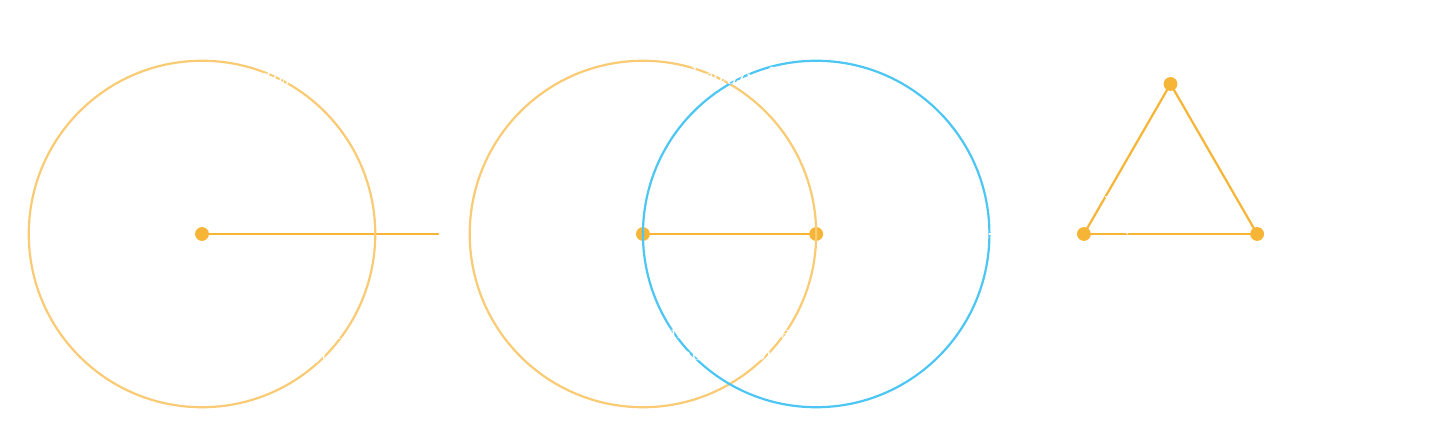
\begin{tikzpicture}[line cap=round, scale=1.0]
% ---------- Panel 1: titik A dan busur pertama ----------
\begin{scope}[shift={(0,0)}]
  \draw[white!60] (-1.2,-1.6) grid[step=0.5] (4.2,2.6);
  \coordinate (A) at (0,0);
  \fill[aksen] (A) circle (2.5pt);
  \node[white, below left, font=\small] at (A) {$A$};
  \draw[aksen, thick] (A) -- (3,0);
  \node[white, below, font=\small] at (1.5,-0.05) {};
  \draw[aksen!70, thick] (A) circle (2.2);
  \node[white, font=\small\itshape, text width=4cm, align=center] at (1.5,2.2) {Langkah 1: busur dari titik $A$};
  \node[white!70, font=\scriptsize, text width=4cm, align=center] at (1.5,-1.4) {Gambar busur berpusat $A$ melewati ruas $AB$.};
\end{scope}
% ---------- Panel 2: busur kedua dari B ----------
\begin{scope}[shift={(5.6,0)}]
  \draw[white!60] (-1.2,-1.6) grid[step=0.5] (4.2,2.6);
  \coordinate (A) at (0,0);
  \coordinate (B) at (2.2,0);
  \draw[aksen, thick] (A) -- (B);
  \fill[aksen] (A) circle (2.5pt); \fill[aksen] (B) circle (2.5pt);
  \node[white, below left, font=\small] at (A) {$A$};
  \node[white, below right, font=\small] at (B) {$B$};
  \draw[aksen!70, thick] (A) circle (2.2);
  \draw[cyan!70, thick] (B) circle (2.2);
  \node[white, font=\small\itshape, text width=4cm, align=center] at (1.5,2.2) {Langkah 2: busur kedua dari $B$};
  \node[white!70, font=\scriptsize, text width=4.2cm, align=center] at (1.5,-1.4) {Busur sama besar dari titik $B$ memotong busur pertama.};
\end{scope}
% ---------- Panel 3: perpotongan C, segitiga sama sisi ----------
\begin{scope}[shift={(11.2,0)}]
  \draw[white!60] (-1.2,-1.6) grid[step=0.5] (4.2,2.6);
  \coordinate (A) at (0,0);
  \coordinate (B) at (2.2,0);
  \coordinate (C) at (1.1, 1.9053);
  \draw[aksen, thick] (A) -- (B);
  \draw[aksen, thick] (A) -- (C) -- (B);
  \fill[aksen] (A) circle (2.5pt); \fill[aksen] (B) circle (2.5pt); \fill[aksen] (C) circle (2.5pt);
  \node[white, below left, font=\small] at (A) {$A$};
  \node[white, below right, font=\small] at (B) {$B$};
  \node[white, above, font=\small] at (C) {$C$};
  % tanda sudut di A
  \draw[white!80] (0.55,0) arc[start angle=0, end angle=60, radius=0.55];
  \node[white, font=\scriptsize] at (0.78,0.34) {$60^\circ$};
  \node[white, font=\small\itshape, text width=4cm, align=center] at (1.5,2.35) {Langkah 3: hubungkan $C$};
  \node[white!70, font=\scriptsize, text width=4.2cm, align=center] at (1.5,-1.4) {Segitiga $ABC$ sama sisi, jadi sudut di $A$ tepat $60^\circ$.};
\end{scope}
\end{tikzpicture}
\end{document}
